\documentclass[11pt, oneside]{article}   	% use "amsart" instead of "article" for AMSLaTeX format
\usepackage{geometry}                		% See geometry.pdf to learn the layout options. There are lots.
\geometry{letterpaper}                   		% ... or a4paper or a5paper or ... 
%\geometry{landscape}                		% Activate for for rotated page geometry
%\usepackage[parfill]{parskip}    		% Activate to begin paragraphs with an empty line rather than an indent
\usepackage{graphicx}
\graphicspath{ {/Users/adeelasaalim/Pictures/} }				% Use pdf, png, jpg, or eps§ with pdflatex; use eps in DVI mode
								% TeX will automatically convert eps --> pdf in pdflatex		
\usepackage{amssymb}

\title{Test Plan}
\author{}
%\date{}							% Activate to display a given date or no date

\begin{document}
\maketitle
\section{Introduction}
%\subsection{}
This test plan has been created to check if our system conforms to all functional requirements and also to specify the types of testing which will be used to validate the functional requirements, action required on failed tests and time line to perform testing of the system.
\section{Objectives and Tasks}
\subsection{Objectives}
The objective of testing our system is to provide adequate testing of functional requirements, validation and behaviour of system under simulated condition. Exhaustive testing of system is not possible but we will use a diverse range of tests to find bugs and errors in the system including unit, functional, error and system testing. System is implemented using java therefore cross platform testing will be performed too. Automation testing will not be possible because most of the methods needs objects to be passed as parameters and their behaviour is changed on every tick of simulation. Testing will be done by running the simulation, observing the agents' behaviour and comparing it with expected behaviour. Debug methods are written to eliminate bugs in the code and exceptions are handled to avoid the crashes.
\subsection{Tasks}
\begin{itemize}
\item Identifying functional requirements and writing the tests cases.
\item Executing tests.
\item Record the failed test cases and reporting them to team.
\item Performing the re-test on failed test cases one bugs are fixed.
\end{itemize}
\section{Scope}
In context to our system, which is implemented using agent-based model it will be tested at three different levels of functionality.
\begin{itemize}
\item \textbf{Agent behaviour: }\hfill \\
Can be checked by changing environment variables around agents.
This forms functional requirements of the system as well. We have two agents in our system. \begin{enumerate}
\item \textbf{Vehicles}\hfill \\
step() method of Vehicle class is the entry point of control into simulation. All methods related to vehicle behaviour are invoked inside this method.\hfill \\
\begin{itemize}
\item \textbf{Test Case1:} Vehicle Impasse\hfill \\
\textit{Expected Output: }This "if condition" in step() method should not be true i.e. no Vehicle should be stuck in impasse.\hfill \\
\textit{Actual Output:} Console output does not print the statement "Vehicle is stuck in impasse. Cannot move...". "if condition" remains false.\hfill \\
\textit{Result:} Passed\hfill \\

	\item \textbf{Test Case 2:}Move towards\hfill \\
	\textit{Input:}Coordinate and displacment\hfill \\
	\textit{Expected Output:}Every vehicle on the network should move to a new coordinate and exception should not be thrown printing on console "Could not move vehicle for some reason.".\hfill \\
	 \textit{Actual Output:}Vehicle moved. No exception thrown.\hfill \\
	 \textit{Result:}Passed
	\item Accelerate: 
	\item Get vehicle ahead
	\item Find best route
	\item Slow down
\end{itemize}

\item \textbf{Traffic Lights}
\begin{itemize}
\item \textbf{Test Case 1:} Traffic Light Green \hfill \\
Expected Output:
Cars should keep moving if traffic light is green.\hfill \\
Actual Output:
Cars did not stop.\hfil \\
Result:
Passed.
\item \textbf{Test Case 2:} Traffic Light Red\hfill \\
 Expected Output: Cars should stop if traffic light is red.\hfill \\
 Actual Output: Cars stops when traffic light is red.\hfill \\
 Result: Passed
 
 \item \textbf{Test Case 3:} Traffic Lights On More Than 2 Roads Junction\hfill \\
 Traffic lights should only be displayed on junctions that contain more than two roads.\hfill \\
 Expected Output: Only junctions with more than two roads display traffic lights.\hfill \\
 Actual Output: Traffic lights are displayed only on more than two road junctions.\hfill \\
 Result: Passed
\end{itemize}

 \end{enumerate}
\item \textbf{Runtime Parameters:} \hfill \\
Elements and data which loads at run time will form part of runtime testing. It will be tested, giving all valid and invalid inputs and check results. Following elements will be tested at run time:
\begin{itemize}
\item \textbf{Test Case 1:} SignalGreenBuilder Implements ContextBuilder\hfill \\
This class contains methods to build the context and initialise all variables required during the simulation execution.\hfil \\
\textit{Input:} Run signalGreen Model, to load user GUI which contains GIS map, Vehicle agents and TrafflicLight Agents.\hfill \\
\textit{Expected Output:} Map should be loaded and displayed along with three different types of vehicles and traffic lights on all junctions that have more than two edges.\hfill \\
\textit{Actual Output:} Map loaded with 100 vehicles which is default value and traffic lights on junctions with more than two edges only.\hfill \\
\textit{Result:} Passed
\item\textbf{Test Case 2:} Number of vehicles\hfill \\
\textit{Input:} Enter a number in "Number of vehicles" field on parameters tab.\hfill \\
4, 0 , -1 and a character given as input.\hfill \\
\textit{Expected Output:} Only entered number of vehicles should appear on road network. No vehicles should appear for negative numbers and characters. \hfill \\
\textit{Actual Output:}  Vehicles are equal to number entered. No vehicles for negative and character input.\hfil \\
\textit{Result:} Passed
\includegraphics{4cars}\hfill \\
\item \textbf{Test Case 3:} No Traffic Lights\hfill \\
"Traffic Lights" on parameters tab, if unchecked traffic lights should not appear on display and cars should not consider traffic lights.\hfill \\
Expected Output: Cars should travel on road without stopping at traffic lights as there are none.\hfill \\
Actual Output: No traffic lights and cars carry on moving on roads.
\end{itemize}
\item \textbf{Overall behaviour of system: }\hfill \\
Checks that all agents of the system produce expected results in a given scenario. This will include testing of agents interaction with other components of environment (roads, traffic lights) when programme will be executed at run time.\hfill \\
\textbf{Test Case 1:} Every junction holds a queue of vehicles running on a particular outward road.\hfill \\
Expected Output of next.printVehiclesQueue(origin):[signalGreen.Vehicle@54008645, signalGreen.Vehicle@1a43b86b] Peek vehicle: signalGreen.Vehicle@54008645\hfill \\
Actual Output: Using probe tool, selecting area which we want to inspect:\hfill \\
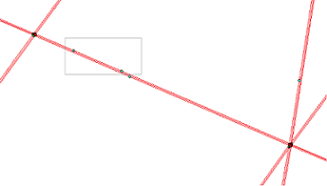
\includegraphics{RoadNetwork}\hfill \\
There are indeed two vehicles running on W 34th St, and their object ID match.
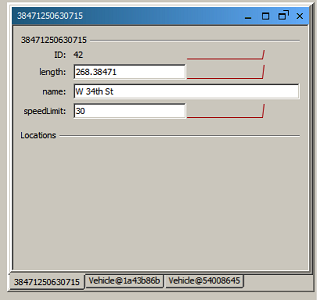
\includegraphics{Sim}\hfill \\
Result: Passed
\end{itemize}
\end{document}  